\clearpage
\onecolumn
\section{RQ3: feature definitions and evaluation}\label{app:ton-protocol}
This supplement gives the feature definitions, evaluation protocol and separate orientation controls supporting RQ3.

\subsection{Source selection, folds and model settings}
The feature study uses 60,251 accepted original A--Z images. The original Kaggle test images duplicate training sources and are not used as an independent test. Five frozen folds separate six blocks of consecutive file numbers, not verified participants. Every representation shares source IDs, labels and held-out partitions. Test folds were inspected during development; this is exploratory validation. The historical feature-cache detector thresholds were not retained. Matching image counts do not establish equivalence with the separately recorded RQ2 detector configuration.

\begin{table}[h]\centering\small
\caption{Feature blocks. D is always retained; S, E and J are independently included or omitted.}
\begin{tabular}{lrp{.70\linewidth}}\toprule
Block & Inputs & Meaning\\\midrule
D & 190 & Normalized distances between image landmarks following Shin.\\
S & 630 & Direction cosines for 210 landmark pairs relative to the image axes; these are not internal joint angles.\\
E & 70 & One-hot categories for the 19 own checks: flexion, spreading, crossing, thumb shape and contact.\\
J & 15 & Fourteen internal angles and one signed thumb deviation from estimated world landmarks. MCP measurements are geometric approximations.\\\bottomrule
\end{tabular}
\end{table}

The eight representations are DS, D, DSE, DE, DSJ, DJ, DSEJ and DEJ. DSEJ contains 905 inputs. E is derived from measured geometry, not from the correct letter. Original images are used without augmentation or right normalization in this factorial comparison. D/S/E/J were recomputed on 390 sources; all 19 one-hot groups were checked across the full cache.

SVM uses an RBF kernel, $C=10$, \texttt{gamma=scale} and balanced classes. LightGBM uses 100 trees, 31 leaves, learning rate 0.1, minimum 20 examples per leaf and seed 42 \citep{ton-lightgbmdocs}. Only J receives median imputation and standardization fitted on the training fold. No representation-specific parameter search is performed. Macro-precision and macro-F1 average equally across A--Z, assigning zero to undefined letter scores.

\begin{table}[h]\centering\small
\caption{Paired changes relative to DS. Net is corrected minus newly introduced errors on the same 60,251 images.}
\begin{tabular}{lrrrrrr}\toprule
 & \multicolumn{3}{c}{SVM} & \multicolumn{3}{c}{LightGBM}\\
Variant & Corrected & Lost & Net & Corrected & Lost & Net\\\midrule
\tonTableInput ton_paired_rows_en.tex
\bottomrule\end{tabular}
\end{table}

The same-coordinate J control uses Shin's image points without aspect correction and shares sources, folds and model profiles. It gains four SVM predictions, compared with 67 using world J. The coordinate source is therefore a relevant alternative explanation.

\clearpage
\subsection{Permutation procedure}
Within each fold, seed 20261107 selects 100 held-out images per letter: 2,600 per fold and 13,000 unique sources in total. Five seeded row permutations move all columns in a feature group together, preserving valid one-hot encodings. Labels and trained models remain fixed. D/S/E/J blocks are tested across the eight variants; the 19 E checks are tested in DSE/DE without J, and E/J families in DSEJ/DEJ. The resulting 3,900 interventions retain precision and F1 drops. Spread over folds/repeats is descriptive, not an independent confidence interval. Related features can substitute for one another, and shuffling can create unusual combinations; importance is not a causal feature ranking \citep{ton-sklearnpermutation}.

\begin{figure}[h]\centering
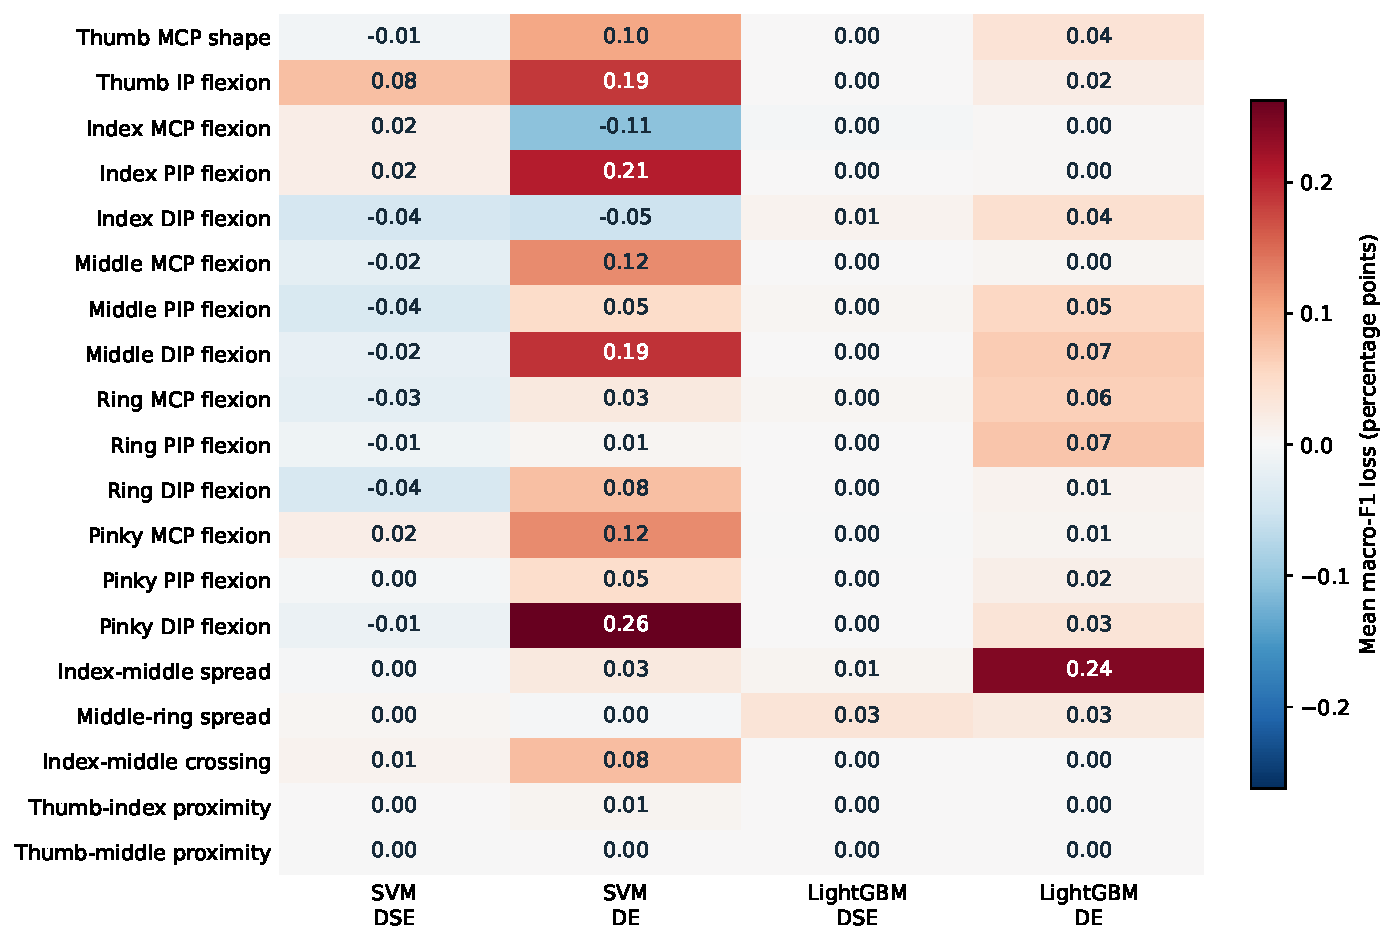
\includegraphics[width=.95\linewidth]{figures/ton_category_importance_en.pdf}
\caption{The 19 own checks, with all one-hot columns of a check shuffled together. Values are mean macro-F1 losses in percentage points over five folds and five shuffles. DSE contains Shin's directions; DE omits them. J is absent in both. Negative losses are retained.}
\label{fig:ton-permutation}
\end{figure}

In DSE, thumb IP flexion has the largest mean F1 loss among E checks for SVM (0.08 percentage points); middle--ring spreading is largest for LightGBM (0.03). These describe fitted-model dependence, not a guaranteed gain from adding a check.

Reproduce with \texttt{python -m RQ3 features} and \texttt{python -m RQ3 coordinate\_control}; commands and output directories are defined in \path{RQ3/workflows.py}. Feature definitions are in \path{research/feature_study.py}; evidence is in \path{results/feature_factorial_01/}. The protocol, 80 fold models, predictions, paired changes, controls, permutation outputs and verification preserve all values underlying the main table. The optional optimized SVM replay checks its outputs against ordinary SVC predictions; it does not alter the experiment.

\clearpage
\section{Own hand features and the inspection tool}\label{app:ton-tool}
The 19 checks comprise 13 flexion checks, two spreading checks, one crossing check, one thumb-shape check and two thumb-tip proximity checks. Multiple categories produce 70 one-hot inputs. They describe estimated landmarks, not independently verified anatomy.

\begin{figure}[h]\centering
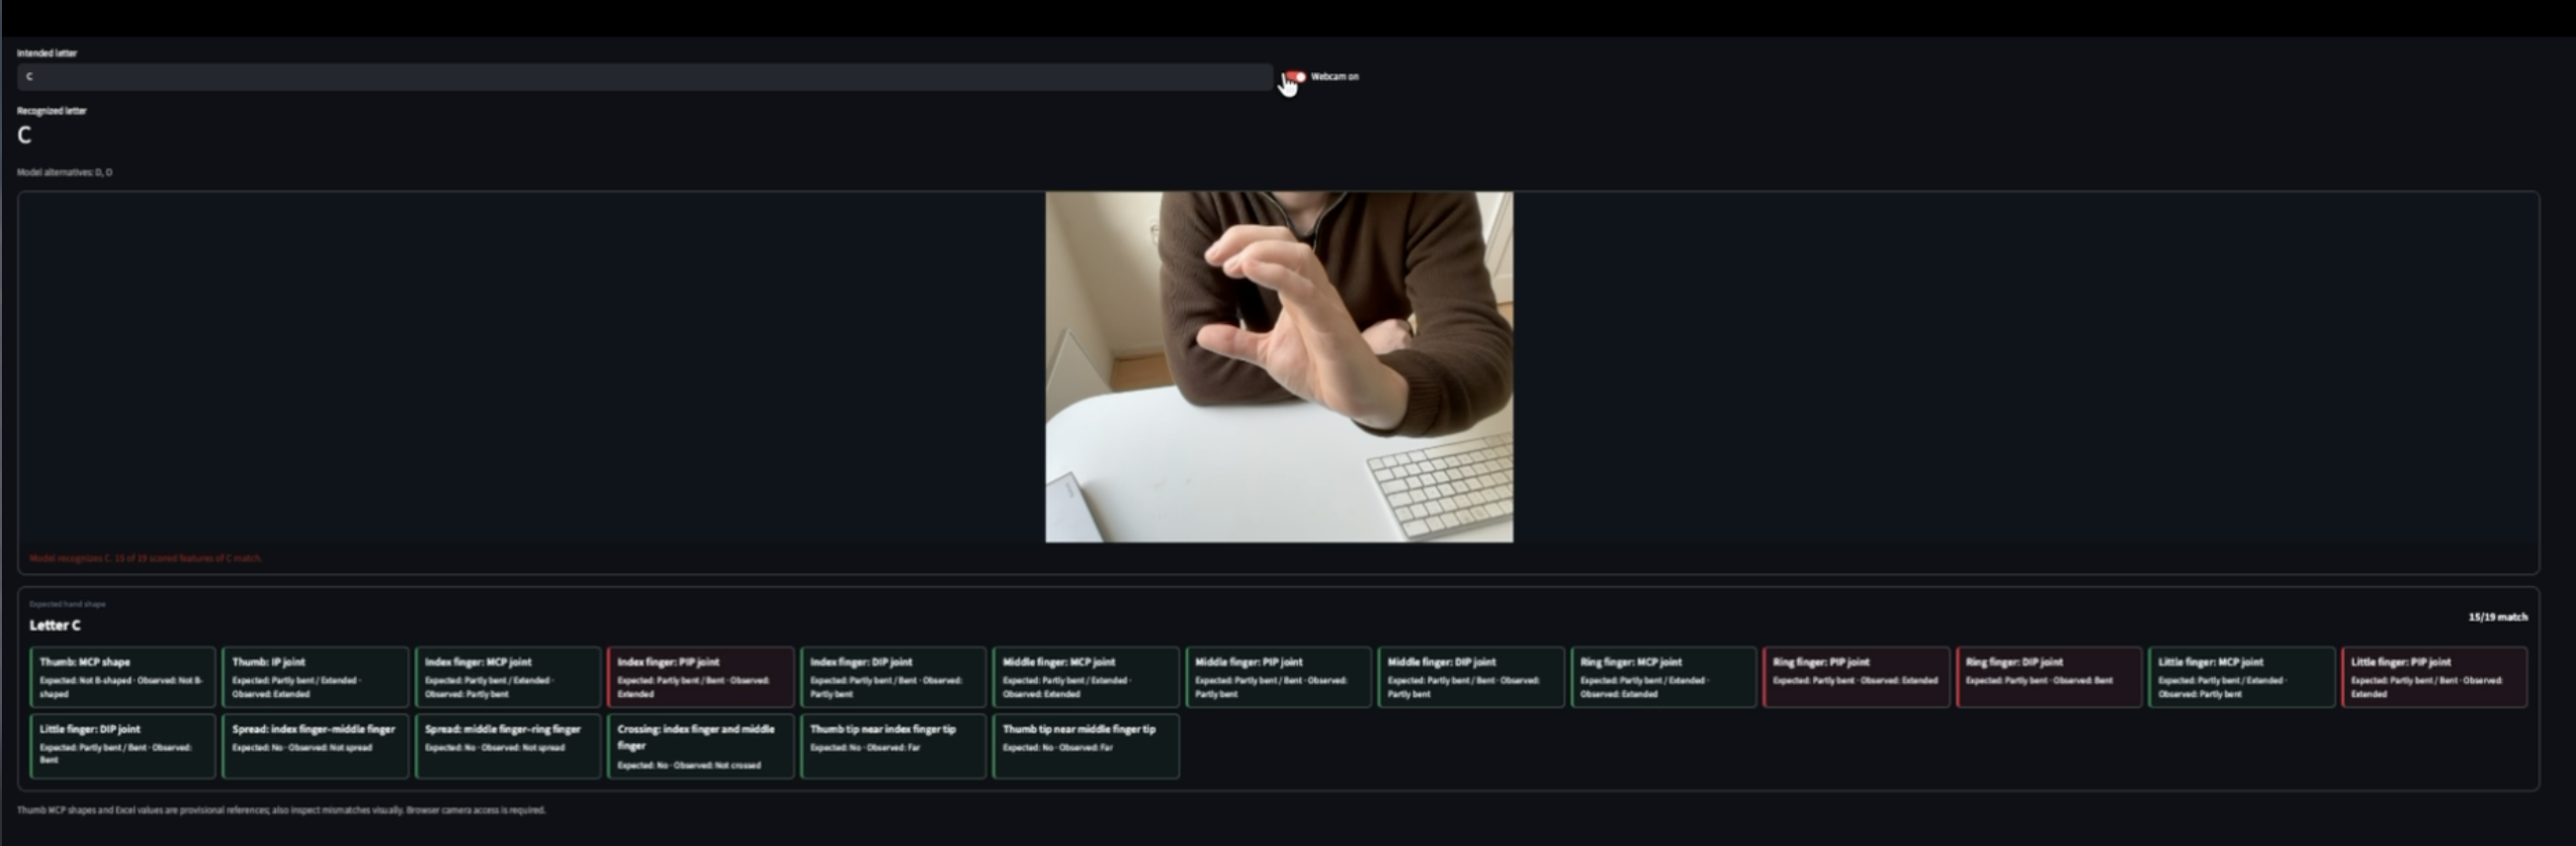
\includegraphics[width=.98\linewidth]{figures/ton_feature_tool_screenshot.png}
\caption{User-supplied feature-tool screenshot. Intended and predicted letter are both C, while only 15 of 19 workbook checks match. The target letter selects expected categories; it does not enter the classifier. Green/red cards indicate agreement with the chosen rules, not confidence in the predicted letter.}
\label{fig:ton-tool}
\end{figure}

\begin{table}[h]\centering\small
\caption{Own feature ideas and their implemented approximations. Thresholds are project choices, stored in \texttt{config/thresholds.json}.}
\begin{tabular}{p{.20\linewidth}p{.70\linewidth}}\toprule
Feature & Measurement and interpretation\\\midrule
Finger flexion (13) & Thumb IP and MCP/PIP/DIP of the other four fingers. A straight joint approaches $180^\circ$. Bent at at most $130^\circ$, extended from $150^\circ$, partly bent between these. Thumb IP uses $80^\circ$ and $155^\circ$.\\
Spreading (2) & Index--middle and middle--ring evaluated separately: normalized lateral gap at least 0.25, depth gap at most 0.6, positive direction cosine, and PIP/DIP angles at least $120^\circ$.\\
Crossing (1) & Index and middle reverse lateral order along their finger profiles, with depth difference at most 0.7 and sufficient extension. Crossing lines in 2D alone are insufficient.\\
Thumb shape (1) & The idea of the thumb across versus beside the palm is approximated by signed thumb-MCP deviation: B-shaped above $16^\circ$ towards the palm. This does not directly measure palm coverage.\\
Thumb-tip proximity (2) & Separate distances to index and middle tips, divided by wrist--middle-MCP length: contact at most 0.1; near up to 0.825; far above this.\\\bottomrule
\end{tabular}
\end{table}

MCP denotes the knuckle, PIP the middle joint, and DIP the end joint; the thumb has an IP joint. The measurements use estimated 3D world points. ``Not spread'' is not the same as touching: the pair can be adjacent, bent or crossed. Direct contact is only checked for the two thumb-tip pairs. ``Not B-shaped'' includes several thumb positions.

The workbook can allow several categories per letter. For ``no contact'', both near and far count as agreement. Unknown measurements are not confirmed agreement; blank reference fields are not scored. In the screenshot, index PIP is observed extended although partly bent/bent is expected, while index--middle is correctly observed not spread. The original screenshot is retained unchanged. The live tool also preserves the actual image, model hash, features and prediction for error analysis.

\clearpage
\section{Exploratory orientation follow-ups}\label{app:ton-orientation}
These short practical explorations tried left/right handling and G/H orientation alongside the main feature study. They retain their own 835-input SVM reference (DSJ) and are not extra arms of the eight-way comparison or independent final validation. The detail below makes the attempted ideas reproducible.

\subsection{RGB mirrors and detector-Right normalization}
Original and horizontally mirrored RGB images are independently detected with IMAGE mode, at most two hands, and detection/presence thresholds 0.5. There are 60,251 accepted originals and 60,201 accepted mirrors. Mirror training adds accepted mirrors of fitting sources while retaining total weight one per source. Original-only preprocessing, numeric gamma and class weights are shared. Sources and their copies remain in the same fold.

Normalization instead uses each detection's own hand label: detector-Left image points receive $x'=1-x$, world points $x'=-x$, then the hand label becomes Right. Other coordinates and anatomical indices remain unchanged; features are recomputed before fitting and inference. This reflection is not a palm-to-back rotation. Detector-Right is unchanged; unknown labels are rejected.

The fixed artificial mixture selects half the source images per letter/fold for RGB mirroring, using seed 20261106 before checking detection success. It contains 60,225 accepted images. Within each presentation all models use the same accepted sources; failed detections are excluded. This is not a verified equal mixture of real left- and right-handed users.

\begin{table}[h]\centering\small
\caption{SVM orientation checks: accepted detections only. P is macro-precision (\%); each test presentation has its own denominator.}
\begin{tabular}{llrrrr}\toprule
Test presentation & Training/input & N & P & Macro-F1 & Correct\\\midrule
\tonTableInput ton_orientation_rows_en.tex
\bottomrule\end{tabular}
\end{table}

On original images, normalization loses 136 correct predictions relative to no change, and mirror training loses 26. On the artificial mixture, normalization improves on no change but remains below mirror training. Detector labels are not independently verified; mirror pairs share pose, person and background. These results do not establish performance for unseen left-handed people. Evidence: \path{results/mirror_01/} and \path{results/handedness_01/}.

\subsection{Why G/H rotation is a different hypothesis}
For usual ASL G/H, the palm faces inward or sideways \citep{ton-vicarsfeedback}. Selected Kaggle training examples show the palm towards the camera. This motivates a possible training/use mismatch, not a demonstrated fault in Shin's learning method; all labels and camera viewpoints have not been independently checked.

A $180^\circ$ camera-$y$ rotation maps wrist-relative coordinates $(x,y,z)$ to $(-x,y,-z)$, with determinant $+1$. Horizontal reflection instead changes only $x$ and has determinant $-1$. A rotated G/H fitting copy and its original each weigh 0.5; other sources retain weight one. The 4,801 G/H sources yield 65,052 fitting rows in the full-data fit. The rotation preserves distances and intrinsic joint measurements; it produces no new RGB image or detector output.

\clearpage
\section{Exploratory G/H checks: artificial versus live views}\label{app:ton-live}
The first test retains all 60,251 accepted original images, including palm-facing G/H labels. The separate artificial control rotates only the 4,801 held-out G/H descriptions; other letters retain their original predictions. Models are not refitted for this test. Neither test independently validates ASL execution. Recognizing an atypical palm-facing G/H is not the intended live-use goal.

\begin{table}[h]\centering\small
\caption{G/H rotation checks over all 26 letters. Both presentations use the same 60,251 sources, but the artificial test replaces G/H geometry.}
\begin{tabular}{llrrr}\toprule
Test descriptions & Training & P (\%) & Macro-F1 & Correct\\\midrule
\tonTableInput ton_gh_rows_en.tex
\bottomrule\end{tabular}
\end{table}

Rotation corrects four original-view errors and introduces five (net $-1$). On the artificial control, it corrects 4,776 errors and loses three (net +4,773); G/H recall reaches 99.47\%/99.45\%. The added geometry is learned, but this is not real hand-back detection. Evidence: \path{results/rotation_GH_y180_01/} and \path{results/gh_occlusion_01/}.

\subsection{Exploratory approximation of occlusion}
A coarse palm ellipsoid and finger volumes are built around source landmarks and rendered with a depth buffer. MediaPipe accepts 64/64 original photographs but 0/64 renders at either 0 or 180 degrees (0/128 total). This rendering route supplies no training detections; known source points are not substituted for failed detector output.

A separate proxy rotates image/world landmarks and adds reproducible Gaussian coordinate noise only to finger joints hidden behind another estimated hand component. The two fixed standard deviations are 2\% and 5\% of wrist--middle-MCP length, scaled separately for image/world coordinates. All 835 features are recomputed. Original fitting weights, folds, preprocessing, gamma and class priors remain fixed. Ten new fold models give no extra gain over pure rotation on either the original or clean artificially rotated test. This is assumed point uncertainty, not a measured distribution of MediaPipe occlusion errors. No independent real hand-back evaluation is implied.

\clearpage
\subsection{Four user-selected live examples}
The original stored landmarks, without redetection, are replayed through both frozen deployment models. All four are accepted detections; model hashes, stored input vectors and recorded predictions are checked. Both hand-back G examples remain H after rotation training. An H changes from Z to H, and a G with the palm visible remains G. Intended letters are user annotations and views are described visually, not expert ASL ground truth. The examples are selected error analysis, not a frequency or accuracy estimate.

\begin{figure}[h]\centering
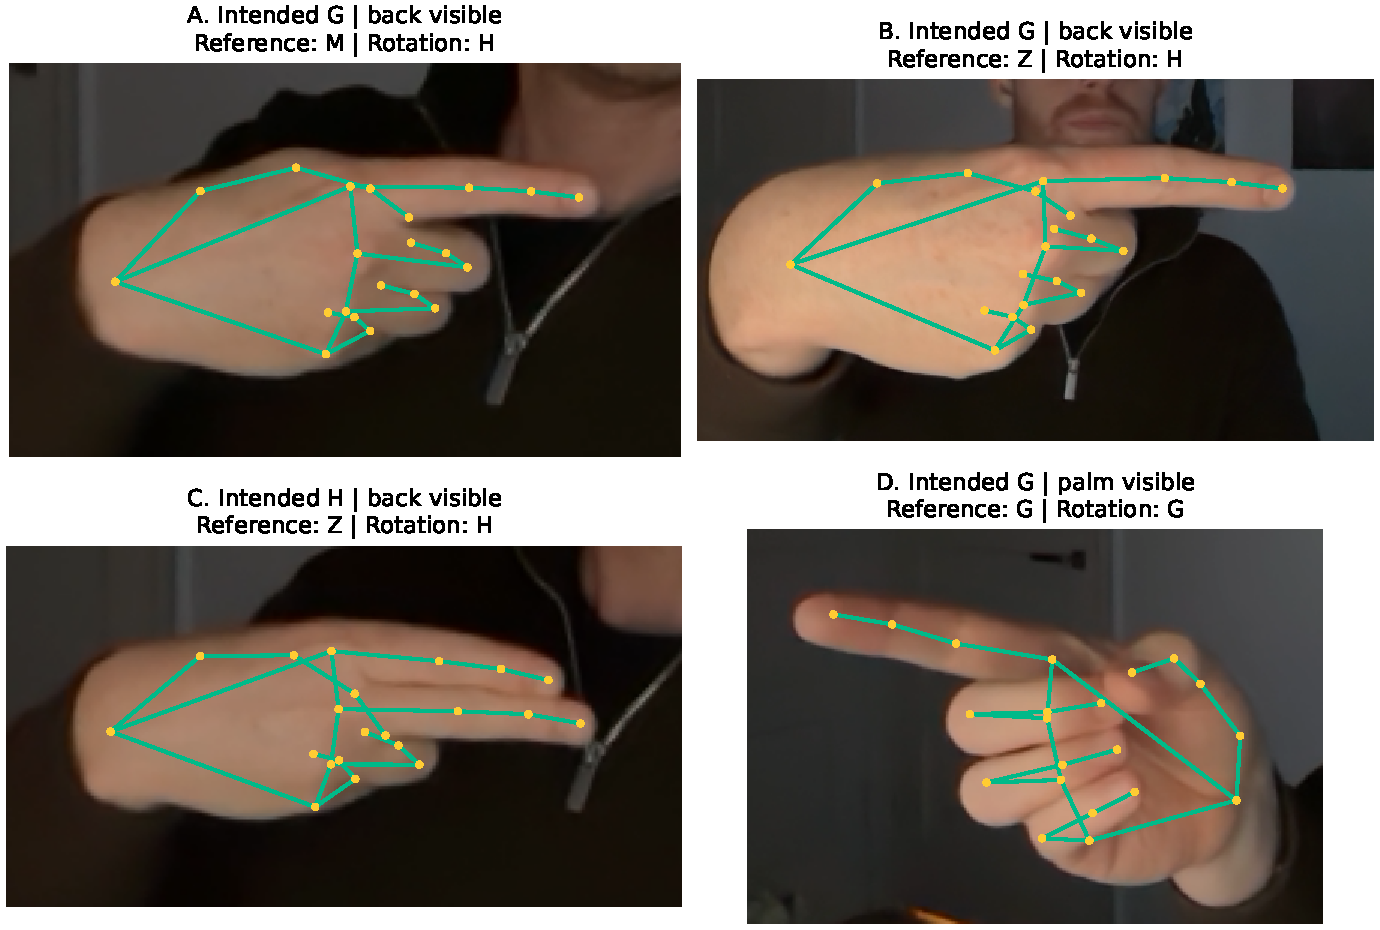
\includegraphics[width=.74\linewidth]{figures/ton_live_examples_en.pdf}
\caption{All four new live examples with stored landmarks. A/B: intended G remains H; C: H is recovered; D: G is recognized with the palm visible. ``Reference'' and ``Rotation'' are model outputs. No image is used for training.}
\label{fig:ton-live}
\end{figure}

The middle-finger DIP estimates in A/B are 161.7 and 164.7 degrees, compared with a G-training median of 113.2 (middle 50\%: 109.2--118.2). Signed thumb deviation is $-1.9$ and $2.7$ degrees versus median 35.9. These are estimated world-point measurements, not true 3D anatomy. Pose, viewpoint and detector error cannot be separated here, nor is one angle proven to cause the classifier error. A rigid rotation preserves the original joint geometry and does not recreate such new detection changes.

The high artificial score therefore does not directly transfer to the live camera. Rotation training is not yet a demonstrated solution to the observed G/H confusion. This observation does not establish the general failure rate. Source IDs, paired outputs, measurements and hashes: \path{results/gh_live_diagnostics_20261107/}.
